\documentclass[aps,prl,twocolumn,superscriptaddress]{revtex4-1}

% the percent sign gives comments in Latex
% top line indicates this is for Physical Review, standard journal format,
% suitable for electronic submission of articles

% the line above is necessary to start any latex document.
% this is one variation that should work for most things.
% if you want double spaceing, use the following:
%
%\documentclass[prd,preprint,letterpaper]{revtex4}
%
% the "preprint" designation will make a wider line
% spacing, good for markup.
\usepackage{graphicx}  % this is the up-to-date package for all figures
\usepackage{amssymb}   % for math
\usepackage{verbatim}  % for the comment environment
\usepackage{color}
\usepackage{gensymb}
\usepackage{amsmath}

\usepackage[section]{placeins}

\usepackage{wrapfig}
\usepackage{hyperref}
\usepackage{titlesec}
\usepackage{amssymb}   % for math
\usepackage{verbatim}  % for the comment environment
\usepackage{color}
\usepackage[nodisplayskipstretch]{setspace}
\usepackage{amsmath}
\usepackage{blindtext}
%\usepackage[pdftex]{graphicx}
\usepackage[outdir=./]{epstopdf}
\usepackage[space]{grffile}
\usepackage{epsfig}
\usepackage[separate-uncertainty=true]{siunitx}
\usepackage{tikz}
\usepackage{pgfgantt}
\usepackage[english]{babel}
\usepackage[utf8]{inputenc}

\titlespacing*{\section}
{0pt}{1\baselineskip}{.5\baselineskip}

\titlespacing*{\subsection}
{0pt}{.5\baselineskip}{.3\baselineskip}



\bibliographystyle{apsrev}


% these are some custom control of the page size and margins
% \topmargin= 0.2in  % these 1st two may be needed for some computers
% \textheight=8.75in
%\textwidth=6.5in
%\oddsidemargin=0cm
%\evensidemargin=0cm

% this is where the actual document itself (rather than control statements) begins:

\begin{document}

% use a style that gives automatic headings
%\pagestyle{headings}



% the \title{} command generates a title.

% the \\ below is used to FORCE a line break in the middle of the sentence--
% otherwise latex computes it for you

\title{NUCRAD Figures}


\author{\textbf{Bryan Yamashiro}}
\author{Christina Nelson}
\author{Corey Mutnik}
\author{Daichi Hiramatsu}

\affiliation{Department of Physics \& Astronomy, \\
University of Hawaii at Manoa,\\
2505 Correa Rd, Honolulu, HI, 96822, USA}
\maketitle




\section{2. Optimal Thickness of NaI Crystal}

\begin{figure}[h!]
  \begin{center}
\centerline{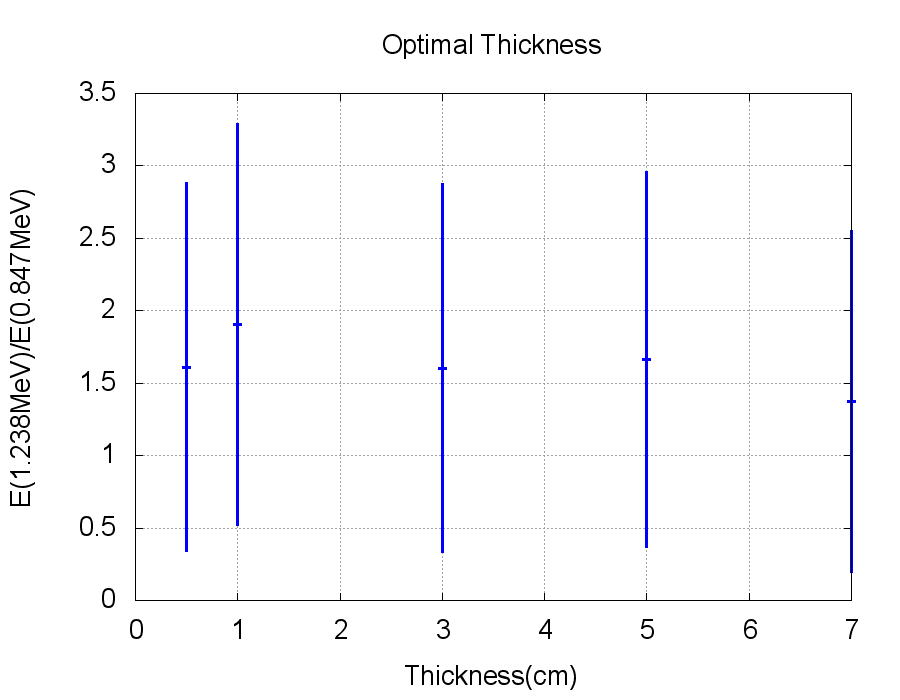
\includegraphics[width=3.5in]{thick.png}}
  \end{center}
\end{figure}

\section{3a. Electron Backscattering and Material Thickness}

\begin{figure}[h!]
  \begin{center}
\centerline{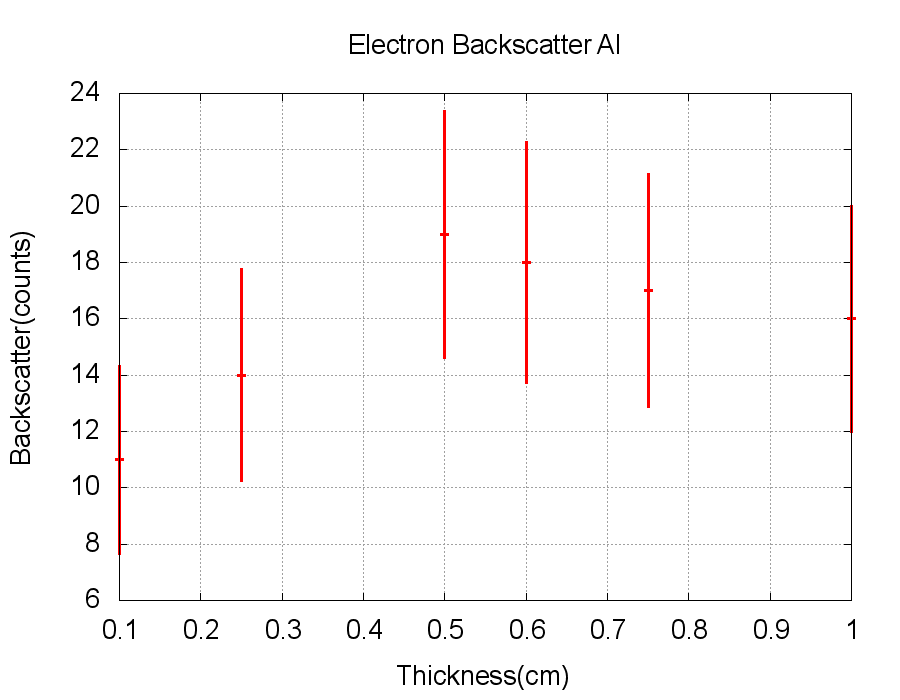
\includegraphics[width=3.5in]{scatteral.png}}
  \end{center}
\end{figure}
\begin{figure}[h!]
  \begin{center}
\centerline{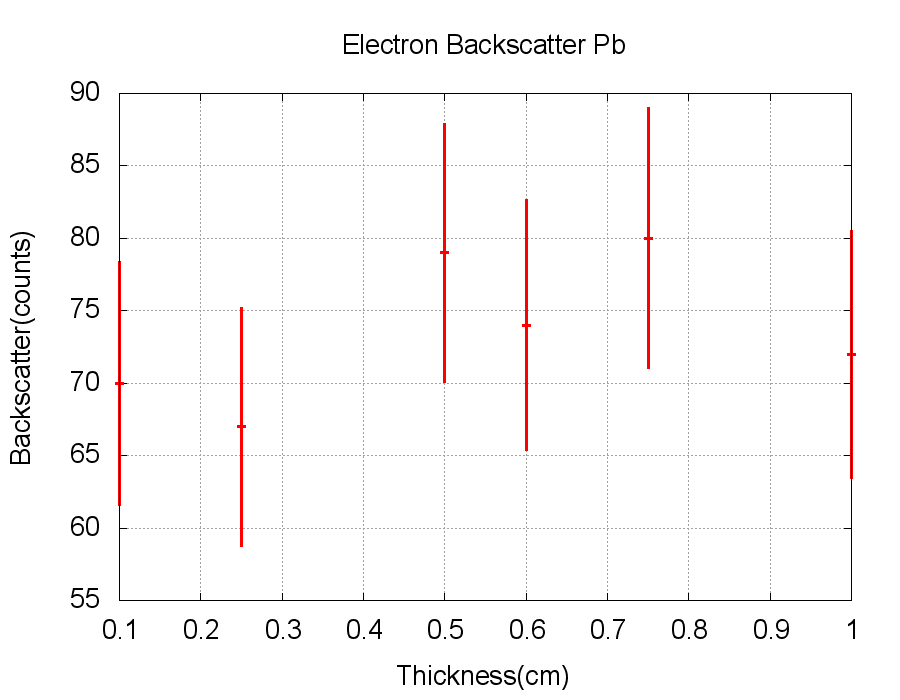
\includegraphics[width=3.5in]{scatterpb.png}}
  \end{center}
\end{figure}

\section{3b. Electron Backscattering and Energy}

\begin{figure}[h!]
  \begin{center}
\centerline{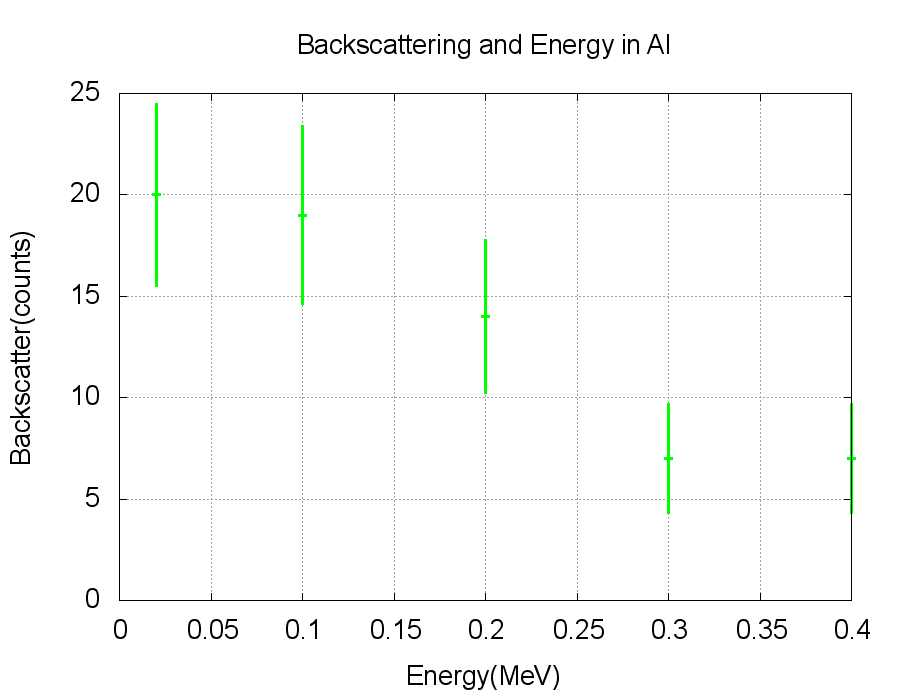
\includegraphics[width=3.5in]{enal.png}}
  \end{center}
\end{figure}
\begin{figure}[h!]
  \begin{center}
\centerline{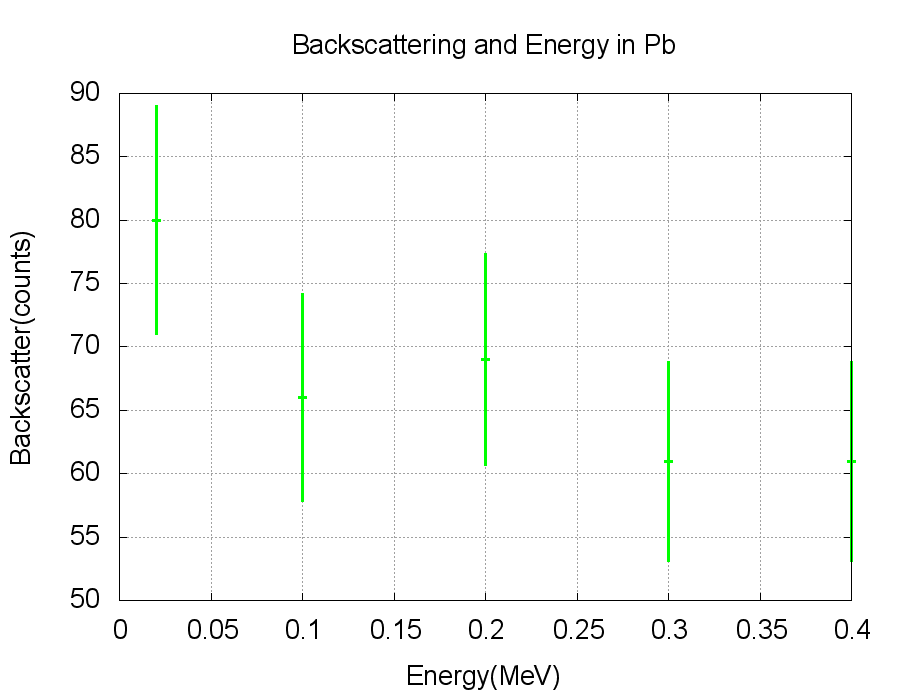
\includegraphics[width=3.5in]{enpb.png}}
  \end{center}
\end{figure}

\section{3c. Electron Backscattering and Material Matter}

\begin{figure}[h!]
  \begin{center}
\centerline{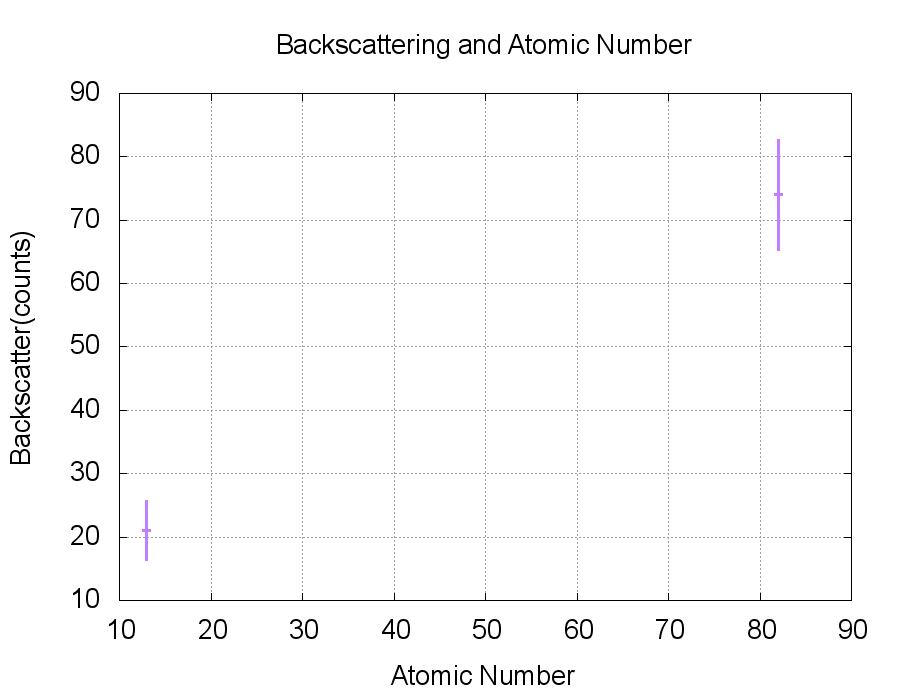
\includegraphics[width=3.5in]{zal.png}}
  \end{center}
\end{figure}
\begin{figure}[h!]
  \begin{center}
\centerline{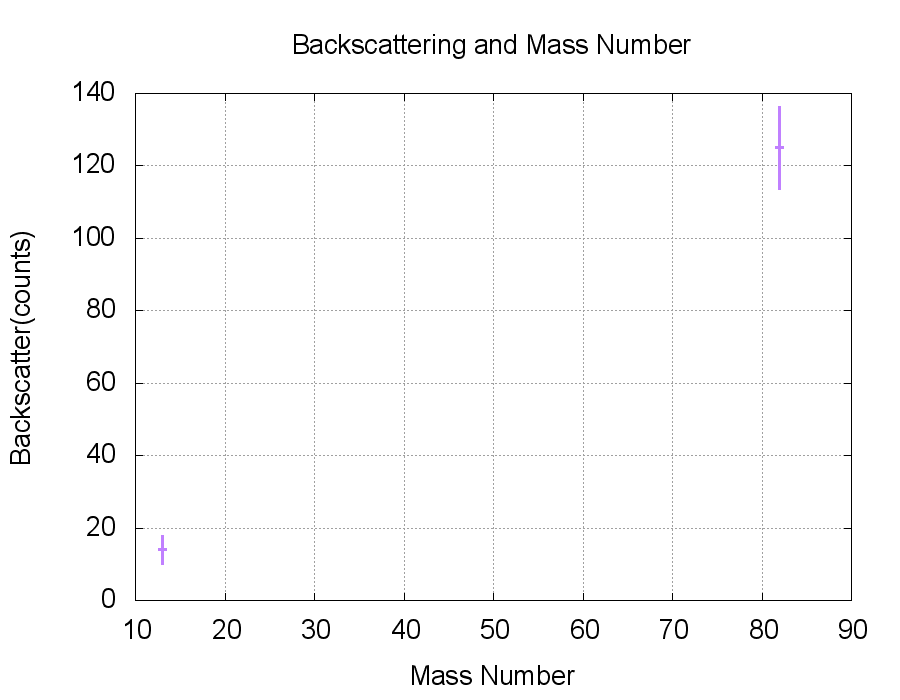
\includegraphics[width=3.5in]{zpb.png}}
  \end{center}
\end{figure}


\end{document}

